\section{Fundamentação Teórica}

	Analisando as forças existentes na gota durante sua subida e sua descida é possível obter a equação para determinação da carga do elétron contido dentro das gotas.
 

\begin{figure}[!htb]
	\centering
	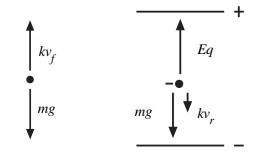
\includegraphics[scale= 1.0]{Esquema}		
	\caption{Forças presentes na gota descendo (direita) e subindo (esquerda)}
	\label{im:Esq}
\end{figure}




	Na subida temos os seguintes termos:
\begin{itemize}
\item k: constante de atrito com o meio;
\item $v_{f}$: velocidade terminal da gota;
\item m: massa da gota;
\item g: gravidade no local;
\end{itemize}
E na descida:
\begin{itemize}
\item E: intensidade do campo elétrico;
\item q: carga do elétron contido na gota;
\item m: massa da gota;
\item g: gravidade no local;
\item k: constante de atrito com o meio;
\item $v_{r}$: velocidade e subida da gota;
\end{itemize}
De acordo com os esquemas presentes na \ref{im:Esq}, temos as seguintes equações:
\begin{equation}
mg = kv_{f}
\end{equation}
\begin{equation}
Eq = mg + kv_{r}
\end{equation}
Eliminando k das duas equações e aplicando a solução para q, é possível reduzir as equações para:
\begin{equation}
q =  \frac{mg(v_{f}+v_{r})}{Ev_{f}}
\label{eq:3}
\end{equation}
Ao aproximar a gota para um formato esférico, é possível escrever a massa como:
\begin{equation}
m =  \frac{4}{3} \pi  a^{3}  \rho
\label{eq:4}
\end{equation}	           
Onde a é o raio da gota e $\rho$ a densidade do óleo. Pela Lei de Stokes, é possível relacionar o raio de um corpo esférico com sua velocidade de queda num meio viscoso (sendo$\eta$ a constante de viscosidade) pela relação:
\begin{equation}
a =  \sqrt{ \frac{9 \eta v_{f}}{2g \rho} }
\label{eq:5}
\end{equation}
Como a velocidade de queda da gota é algo entre 0.01 e 0.001 cm/s, a viscosidade deve ser multiplicada por um fato de correção pois a Lei de Stokes funciona para velocidades maiores do que 0.1 cm/s tal que:
\begin{equation}
\eta_{f} = \eta \left( \frac{1}{1+ \frac{b}{pa} } \right)
\label{eq:6}
\end{equation}
Onde b é uma constante, p é a pressão atmosférica e a o raio da esfera calculado em \ref{eq:5}. Substituindo o $\eta_{f}$ da equação \ref{eq:6} na equação \ref{eq:5},
\begin{equation}
a= \sqrt{ \eta  \frac{9v_{f}}{2gp}  \left( \frac{1}{1+ \frac{b}{pa} } \right)}
\end{equation}
\begin{equation}
a= \sqrt{ \eta  \frac{9v_{f}}{2gp}  \left( \frac{b}{pa+b} \right)}
\end{equation}
\begin{equation}
a =  \sqrt{\left(\frac{b}{2p}\right)^2 +  \frac{9\eta v_{f}}{2gp} } 
\end{equation}
Como o segundo termo da raiz é muito pequeno e comparação às dimensões da gota, o valor do raio da esfera pode ser aproximado para:
\begin{equation}
a = \frac{b}{2p}
\label{eq:10}
\end{equation}
Substituindo as equações \ref{eq:4}, \ref{eq:5} e \ref{eq:6} na equação \ref{eq:3}:

\begin{equation}
q = 6\pi \sqrt{ \frac{9\eta^{3}}{2gp \left(1+ \frac{b}{pa} \right)^{3} } (v_{f} + v_{r})\sqrt{v_{f}}}
\label{eq:11}
\end{equation}

Substituindo as equações \ref{eq:10} e \ref{eq:6} na equação \ref{eq:11}, tem-se a equação geral para determinação da carga do elétron que é
\begin{equation}
q = \left[400\pi d \left(\frac{1}{gp}\left[\frac{9\eta}{2}\right]^{3}\right)^{\frac{1}{2}}\right] \times \left[\left(\frac{1}{1+\frac{b}{pa}}\right)^{\frac{3}{2}}\right] \times \left[\frac{v_{f}+v_{r}\sqrt{v_{f}}}{V}\right]
\end{equation}
Da equação acima, os termos do primeiro membro são definidos para cada conjunto experimental, do segundo membro para cada gota e do terceiro membro para cada mudança na carga das gotas.
Adequando a equação para a montagem experimental utilizada, a expressão é reduzida para:
\begin{equation}
q = \frac{mg(v_{f} + v_{r})}{Ev_{f}}
\end{equation}
\begin{equation}
q = \frac{4}{3} \pi \rho g \left[\sqrt{\left(\frac{b}{2p}\right)^{2} + \frac{9\eta v_{f}}{2g\rho}} - \frac{b}{2p} \right]^{3} \times \frac{v_{f} + v_{r}}{Ev_{f}}
\label{eq:14}
\end{equation}







	
